\documentclass{article}
  \usepackage{amsmath}
  \usepackage{amssymb}
  \usepackage{graphicx}
  \usepackage{float}
  \usepackage{setspace}
  \usepackage{verbatim}
\topmargin=-1.2cm \oddsidemargin=0.1cm \evensidemargin=0.1cm
\textwidth=16 true cm \textheight=23 true cm

\font\euler=EUSM10 \font\eulers=EUSM7

\begin{document}
\title{ECON 3160 Game Theory \\Assignment $4^{\text{st}}$}
\author{{\normalsize Leonard Sheng(SHENG, Hao), 1155035947, via \LaTeX}}
\date{\today}

\maketitle

\def \Pr{{\rm Pr}}

\baselineskip 0.6cm
\begin{description}
    \item[8.6 The three mountains:]{\bf Answer:}\\
    Let's make You the row player and Barbara the column player.\\
    The game can be roughly graphed like this:
    \begin{center}
                    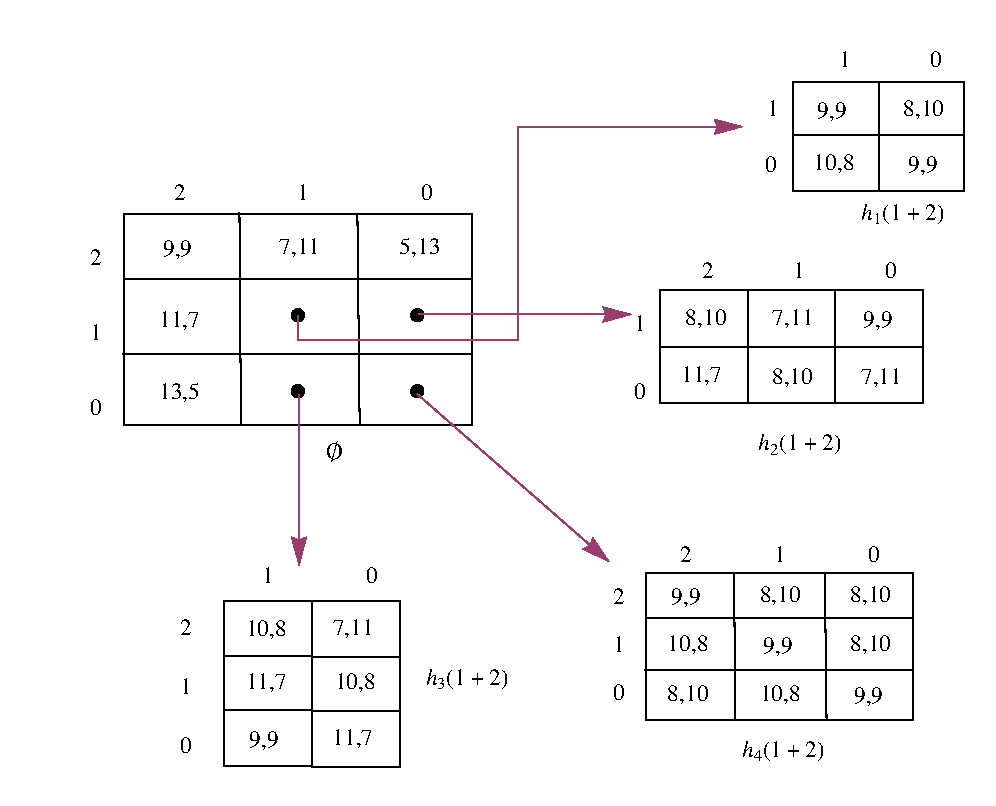
\includegraphics[angle=0, width=0.8\textwidth]{ECON3160A4P1}\\
                    {\bf Figure 8.6} Graphical representation of {\it The three mountains}
    \end{center}
    *Since the 2 unit of energy must be divided over these 3 days, both you and Barbara only need to make choice on the first and second day of this competition.\\
    **Whenever one of you have spent all your energy on the first day, you (or she) don't need to make a decision on the next day. There is no longer any uncertainty in his or her strategy. Thus, we can calculate the utility his or her opponent will get for each of strategies, picking up the best response and writing down the pay-off directly.

    We use {\bf Backwards order of elimination} to solve the problem.

    The full decision problem at $h_1$ are depicted in Table 8.6.1.
    \begin{center}
              % Table generated by Excel2LaTeX from sheet '8.6 h4'
        \begin{tabular}{ccc}
        \hline
        \hline
                   &          $1_1$ &          $0_1$ \\
        \hline
                 $1_1$ &        9,9 &       8,10 \\

                 $0_1$ &       10,8 &        9,9 \\
        \hline
        \end{tabular}

        {\bf Table 8.6.1} Simplified full decision problem at $h_1$.
    \end{center}
     Within $\Gamma ^0\left(h_1\right)$, the groups of strategies $1_1$ are strictly dominated for you and Barbara. We eliminate these strategies.
    \begin{center}
      % Table generated by Excel2LaTeX from sheet '8.6 h4'
        \begin{tabular}{cc}
        \hline
        \hline
                   &          $0_1$ \\
        \hline
                 $0_1$ &        9,9 \\
        \hline
        \end{tabular}

        {\bf Table 8.6.2} Reduced decision problem at $h_1$.
    \end{center}



    The full decision problem at $h_4$ are depicted in Table 8.6.3.
    \begin{center}
              % Table generated by Excel2LaTeX from sheet '8.6 h4'
        \begin{tabular}{cccc}
        \hline
        \hline
                   &          $2_4$ &          $1_4$&          $0_4$ \\
        \hline
                 $2_4$ &        9,9 &       8,10 &       8,10 \\

                 $1_4$ &       10,8 &        9,9 &       8,10 \\

                 $0_4$ &       10,8 &       10,8 &        9,9 \\
        \hline
        \end{tabular}

        {\bf Table 8.6.3} Simplified full decision problem at $h_4$.
    \end{center}
    By eliminating strictly dominated strategies, we get the reduced decision problem:
    \begin{center}
              % Table generated by Excel2LaTeX from sheet '8.6 h4'
        \begin{tabular}{cc}
        \hline
        \hline
                   &          $0_4$ \\
        \hline
                 $0_4$ &        9,9 \\
        \hline
        \end{tabular}

        {\bf Table 8.6.4} Reduced decision problem at $h_4$.
    \end{center}

    By eliminating strictly dominated strategies in $\Gamma ^0\left(h_2\right)$, we get the reduced decision problem:
    \begin{center}
      % Table generated by Excel2LaTeX from sheet '8.6 h4'
        \begin{tabular}{ccc}
        \hline
        \hline
                   &          $1_2$ &          $0_2$ \\
        \hline
                 $1_2$ &       7,11 &        9,9 \\

                 $0_2$ &       8,10 &       7,11 \\
        \hline
        \end{tabular}

        {\bf Table 8.6.5} Reduced decision problem at $h_2$.
    \end{center}

    By eliminating strictly dominated strategies in $\Gamma ^0\left(h_3\right)$, we get the reduced decision problem:
     \begin{center}
          % Table generated by Excel2LaTeX from sheet '8.6 h4'
        \begin{tabular}{ccc}
        \hline
        \hline
                   &          $1_3$ &          $0_3$ \\
        \hline
                 $1_3$ &       11,7 &       10,8 \\

                 $0_3$ &        9,9 &       11,7 \\
        \hline
        \end{tabular}

        {\bf Table 8.6.6} Reduced decision problem at $h_3$.
    \end{center}

    Now, we can move to the beginning of the game. By eliminating the strategies eliminated above, we get the reduced decision problem of $\emptyset$.
    \begin{center}
      % Table generated by Excel2LaTeX from sheet '8.6 h4'
        \begin{tabular}{cccccc}
        \hline
        \hline
                   &          $2_0$ &  ($1_0, 0_1, 1_3$) &  ($1_0, 0_1, 0_3$) &  ($0_0, 1_2, 0_4$) &  ($0_0, 0_2, 0_4$) \\
        \hline
                 $2_0$ &        9,9 &       7,11 &       7,11 &       5,13 &       5,13 \\

         ($1_0, 0_1, 1_2$) &       11,7 &        9,9 &        9,9 &       7,11 &        9,9 \\

         ($1_0, 0_1, 0_2$) &       11,7 &        9,9 &        9,9 &       8,10 &       7,11 \\

         ($0_0, 1_3, 0_4$) &       13,5 &       11,7 &       10,8 &        9,9 &        9,9 \\

         ($0_0, 0_3, 0_4$) &       13,5 &        9,9 &       11.7 &        9,9 &        9,9 \\
        \hline
        \end{tabular}

         {\bf Table 8.6.7} Reduced decision problem at $\emptyset$.
    \end{center}


    \begin{center}
      % Table generated by Excel2LaTeX from sheet '8.6 h4'
        \begin{tabular}{cccc}
        \hline
        \hline
                   &  ($1_0, 0_1, 1_3$) &  ($0_0, 1_2, 0_4$) &   ($0_0, 0_2, 0_4$) \\
        \hline
         ($1_0, 0_1, 1_2$) &        9,9 &       7,11 &        9,9 \\

         ($0_0, 1_3, 0_4$) &       11,7 &        9,9 &        9,9 \\

         ($0_0, 0_3, 0_4$) &        9,9 &        9,9 &        9,9 \\
        \hline
        \end{tabular}

        {\bf Table 8.6.8} Final decision problem at $\emptyset$.

    \end{center}
    At this stage, we can answer these two questions:\\
    {\bf (a):}You can rationally choose strategies of ($1_0, 0_1, 1_3$), ($0_0, 1_2, 0_4$) and ($0_0, 0_2, 0_4$) under common belief in future rationality. This means you should consume 1 or 0 unit of energy rationally during the first stage under common belief in future rationality.\\
    {\bf (b):}I would really pick up the second, namely ($0_0, 1_2, 0_4$). Although the other two strategies are not strictly dominated, they are dominated by the ($0_0, 1_2, 0_4$). Suppose a type of you are now assigning possibility over the three strategies your opponent can rationally make under common belief in future rationality, once you give his(her) strategy ($1_0, 0_1, 1_2$) positive possibility (which is likely to happen in the real life, say, you know he(her) is a person who likes to have an edge from the first. ), only ($1_0, 0_1, 1_3$) can rationally be made. Of course, this type is consist with common belief in future rationality.
    \newpage
    \item[8.7 The Walkin' Fridge:]{\bf Answer:}\\
    Since this game has {\bf perfect information} ,we use {\bf Backward induction} to solve this problem.
    {\bf (a):}
    At the third stage, Chris tries to maximize his utility given your and Barbara's choices:
    \begin{align}
      &\text{Max}\left\{U_C=I_c-C_c={abc}-\frac{c^3}{3}\right\},s.t.0\leq c\leq 200\\
      \intertext{,which gives us:}
      &c=\sqrt{\text{ab}}\in [0,200]
    \intertext{At the second stage, Barbara tries to maximize her utility given your choice. That is:}
      &\text{Max}\left\{U_b=I_b-C_b=({ab})^{\frac{3}{2}}-\frac{b^3}{3}\right\},s.t.0\leq b\leq 200 \\
        \intertext{,which gives us:}
      &b=\left(\frac{3}{2}\right)^{\frac{2}{3}}a\in [0,200]
     \intertext{Finally, when we move to the beginning of the game, the decision problem for you is:}
      &\text{Max}\left\{U_a=\frac{7}{6}a^3\right\},s.t.0\leq a\leq 100 \\
        \intertext{,which gives your optimal stragety under common belief of your opponents' future rationality:}
      &a=100
    \end{align}
    Also, under common belief of your opponents' future rationality,\\ you will expect Barbara dedicates $\left(\frac{3}{2}\right)^{\frac{2}{3}}\cdot 100$ days, and Chris dedicates $\left(\frac{3}{2}\right)^{\frac{1}{3}}\cdot 100$ days.\\\\\\
    {\bf (b):}At the third stage, Chris tries to maximize his utility given your and Barbara's choices:
    \begin{align}
      &\text{Max}\left\{U_C=I_c-C_c={abc}-c^3\right\},s.t.0\leq c\leq 200
      \intertext{,which gives us:}
      &c=\sqrt{\frac{{ab}}{3}}\in [0,200]
    \intertext{At the second stage, Barbara tries to maximize her utility given your choice. That is:}
      &\text{Max}\left\{U_b=I_b-C_b=\frac{\sqrt{3}}{3}(\text{ab})^{\frac{3}{2}}-b^3\right\},s.t.0\leq b\leq 200 \\
        \intertext{,which gives us:}
      &b=\left(\frac{\sqrt{3}}{6}\right)^{\frac{2}{3}}a\in [0,200]
     \intertext{Finally, when we move to the beginning of the game, the decision problem for you is:}
      &\text{Max}\left\{U_a=-\frac{5}{6}a^3\right\},s.t.0\leq a\leq 100 \\
        \intertext{,which gives your optimal stragety under common belief of your opponents' future rationality:}
      &a=0
    \end{align}
    Also, under common belief of your opponents' future rationality,\\ you will expect Barbara dedicates $0$ day, and Chris dedicates $0$ day.\\\\\\
    {\bf (c):}
    After some tedious calculation like part(a) and (b), finally we get the reduced decision problem for You:

    \begin{center}
                    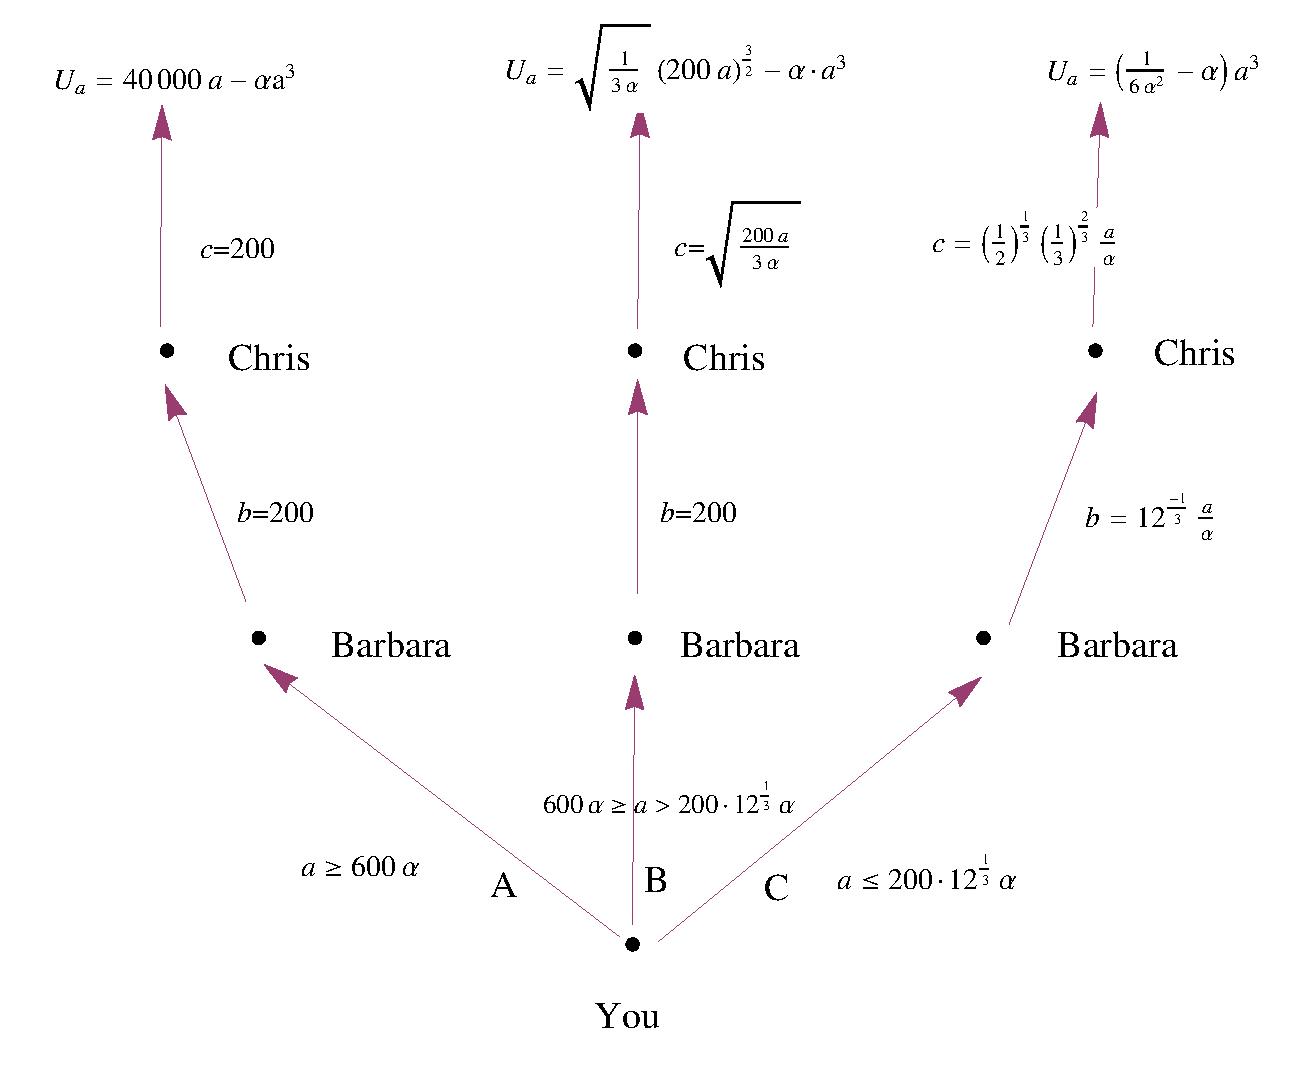
\includegraphics[angle=0, width=0.8\textwidth]{ECON3160A4P2}\\
                    {\bf Figure 8.7.1} Reduced decision problem for You of {\it The Walkin' Fridge}
    \end{center}
    where we list three possible strategy groups of You in the first stage, namely, $A$, $B$ and $C$, which may lead to different response of Barbara and Chris in the sense of existence of corner solution.\\

    Then, we try to optimize your choice by looking into each possibility.
    First, we maximize your utility among each of your strategy groups, which gives us:
    \begin{align}
      U_{a,a\in A,\max }&=(4-\alpha )\cdot 10^6\\
      a _{A,\max }&=100\\
      U_{a,a\in B,\max }&=\left(2\sqrt{\frac{2}{3\alpha }}-\alpha \right)\cdot 10^6\\
      a _{B,\max }&=100\\
      U_{a,a\in C,\max }&=\begin{cases}
 0 & \alpha \geq \left(\frac{1}{6}\right)^{\frac{1}{3}} \\
 \left(\frac{1}{6\alpha ^2}-\alpha \right)\cdot 10^6 & 12^{-\frac{1}{3}}<\alpha <\left(\frac{1}{6}\right)^{\frac{1}{3}} \\
 \left(\frac{1}{6\alpha ^2}-\alpha \right)\cdot 9.6\cdot 10^6\alpha ^3 & \alpha \leq 12^{-\frac{1}{3}}
\end{cases}\\
       a_{C,\max }&=\begin{cases}
 0 & \alpha >\left(\frac{1}{6}\right)^{\frac{1}{3}} \\
 \forall a_0\in [0,100] & \alpha =\left(\frac{1}{6}\right)^{\frac{1}{3}} \\
 100 & 12^{-\frac{1}{3}}<\alpha <\left(\frac{1}{6}\right)^{\frac{1}{3}} \\
 200\cdot 12^{\frac{1}{3}}\alpha  & \alpha \leq 12^{-\frac{1}{3}}
\end{cases}
    \end{align}
    Then ,since Your choice $a$ need to be a real number between zero and 100, we can look into three basic possibilities of $\alpha$ respectively:
    \begin{description}
      \item[i).$\alpha \leq \frac{1}{6}$]:These three strategy groups are all possible for you.\\
        Plot these three utility functions:
         \begin{center}
                    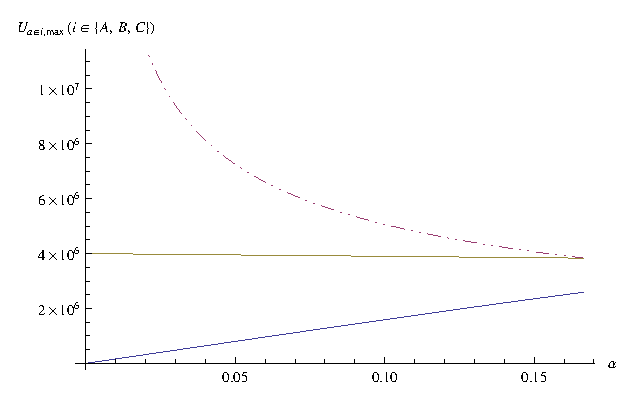
\includegraphics[angle=0, width=0.8\textwidth]{ECON3160A4P21}\\
                    {\bf Figure 8.7.2} Utility of local optimal strategy among your strategy groups in (i)
        \end{center}
        We can see the dashed one, that is the local optimal strategy in strategy groups $B$ is the highest one.
      \item[ii).$\frac{1}{6}<\alpha \leq \frac{12^{\frac{-1}{3}}}{2}$]:Only strategy groups $B$ and $C$ are possible for you.\\
        Plot these two utility functions:
         \begin{center}
                    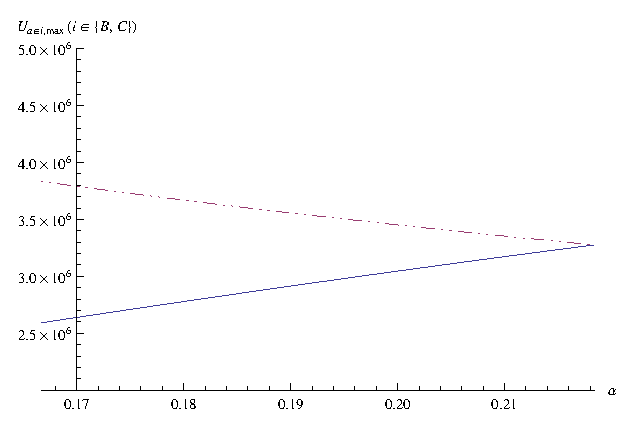
\includegraphics[angle=0, width=0.8\textwidth]{ECON3160A4P22}\\
                    {\bf Figure 8.7.3} Utility of local optimal strategy among your strategy groups in (ii)
        \end{center}
        We can see the dashed one, that is still the local optimal strategy in strategy groups $C$ is the highest one.
      \item[ii).$\frac{12^{\frac{-1}{3}}}{2}<\alpha$]:Only strategy groups $B$ are possible for you.
    \end{description}
        In sum, the number of days you will rationally dedicate to the Walkin' Fridge project under common belief in future rationality is:
        \begin{align}
          a^*=\begin{cases}
         0 & \alpha >\left(\frac{1}{6}\right)^{\frac{1}{3}} \\
         \forall a_0\in [0,100] & \alpha =\left(\frac{1}{6}\right)^{\frac{1}{3}} \\
         100 & \alpha <\left(\frac{1}{6}\right)^{\frac{1}{3}}
            \end{cases}
        \end{align}
        And under common belief in future rationality, you will expect Barbara and Chris dedicate days:
        \begin{align}
          b^*=\begin{cases}
             0 & \alpha >\left(\frac{1}{6}\right)^{\frac{1}{3}} \\
             12^{-\frac{1}{3}}\cdot a_0 & \alpha =\left(\frac{1}{6}\right)^{\frac{1}{3}} \\
             12^{\frac{-1}{3}}\cdot 100 & \frac{12^{\frac{-1}{3}}}{2}\leq \alpha <\left(\frac{1}{6}\right)^{\frac{1}{3}} \\
             200 & \alpha <\frac{12^{\frac{-1}{3}}}{2}
            \end{cases}\\
            c^*=\begin{cases}
             0 & \alpha >\left(\frac{1}{6}\right)^{\frac{1}{3}} \\
             \left(\frac{3}{2}\right)^{\frac{1}{3}}\cdot a_0 & \alpha =\left(\frac{1}{6}\right)^{\frac{1}{3}} \\
             \left(\frac{3}{2}\right)^{\frac{1}{3}}\cdot 100 & \frac{12^{\frac{-1}{3}}}{2}\leq \alpha <\left(\frac{1}{6}\right)^{\frac{1}{3}} \\
             \sqrt{\frac{20000}{3\alpha }} & \frac{1}{6}\leq \alpha <\frac{12^{\frac{-1}{3}}}{2} \\
             200 & \alpha <\frac{1}{6}
            \end{cases}
        \end{align}

    \newpage
    \item[8.9 Repeated games:]{\bf Answer:}\\
    {\bf (c):}To make things simple, we will construct a game of two players.\\
    Although we haven't proof the statement in part (a), let's suppose it's true. Thus, we should first construct a game where your opponent have at least two choices that survive the iterated elimination of strictly dominated choice in the static game. Suppose you are the player 1(the player we concern about) and both of you and your opponent have two choices in the static game. The pay-off are given as:
    \begin{center}
                    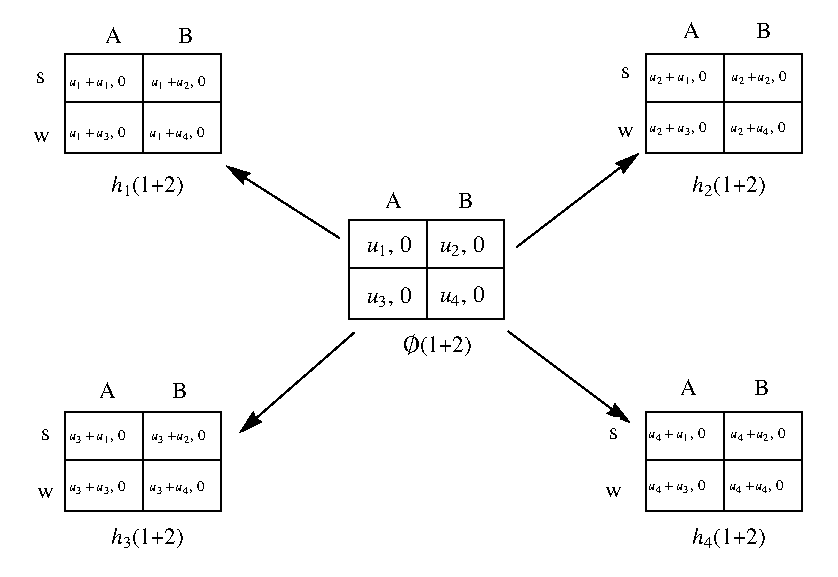
\includegraphics[angle=0, width=0.8\textwidth]{ECON3160A4P3}\\
                    {\bf Figure 8.9.1} Graphical representation of {\it Repeated games}
    \end{center}
    where $s$ represents your strictly dominating choice in the static game, while $w$ represents your strictly dominated choice in the static game. So, we have:
    \begin{align}
      &u_1>u_3\\
      &u_2>u_4
    \end{align}
    Since your opponent always gets utility of zero, all of his(her) strategies are rational under any belief at the first period; all of his(her) strategies are rational under any conditional belief at the second period as long as they can lead to such information sets. We can form a type of him(her) arbitrarily, which can justify all of his(her) strategies. As a result, all of your type express 1-fold belief in opponent's future rationality. what we need to do now is to construct a type of your opponent that express 1-fold belief in his(her) opponent's future rationality.\\
    When you reached the second game, that is, the information set of $h_1$, $h_2$, $h_3$ and $h_4$, your strategy groups $w_1$, $w_2$, $w_3$ and $w_4$ are strictly dominated by your strategy groups $s_1$, $s_2$, $s_3$ and $s_4$, respectively.\\
    So, when we getting back to the first period of the game, with your strategy groups eliminated, we have the reduced decision problem:
    \begin{center}
      % Table generated by Excel2LaTeX from sheet '8.10c'
        \begin{tabular}{cccc}
        \hline
        \hline
                   & ($A_0,A_1,A_3$) & ($A_0,B_1,A_3$) &         ... \\
        \hline
        ($s_0,s_1,s_2$) &     2$u_1$,0 &  $u_1+u_2$,0 &          ... \\

        ($w_0,s_3,s_4$) &  $u_1+u_3$,0 &  $u_1+u_3$,0 &         ... \\
        \hline
        \end{tabular}

    {\bf Table 8.9.1} Reduced decision problem at $\emptyset$
    \end{center}
    To prevent strategy ($w_0,s_3,s_4$) eventually being eliminated, we only need to set it optimal for some of your belief at $\emptyset$. For example, let's set $$u_1+u_3>u_1+u_2$$, that is under the belief of your opponent's strategy ($A_0,B_1,A_3$). $u_3>u_1$ can be satisfied simultaneously with $u_1>u_3$ and $u_2>u_4$. Since ($w_0,s_3,s_4$) has already been the optimal strategy when you found you are in $h_3$ or $h_4$, it's optimal for some of your types that express 1-fold belief of your opponent's future rationality.\\

    Precisely, we can give an example of static game $G$ and an epistemic model where the choice $w$ can be rationally chosen under common belief in future rationality at $\emptyset$ :
    \begin{center}
      % Table generated by Excel2LaTeX from sheet '8.10c'
        \begin{tabular}{rrcc}

                   &            & \multicolumn{ 2}{c}{{\bf Your opponent}} \\

                   &            &          A &          B \\

        \multicolumn{ 1}{c}{{\bf You}} &          s &        3,0 &        1,0 \\

        \multicolumn{ 1}{c}{{\bf }} &          w &        2,0 &        0,0 \\

        \end{tabular}

        {\bf Table 8.9.2} One possible pay-off matrix of game $G$ in {\it 8.9 Repeated games}\\
    \end{center}




    \begin{center}
      % Table generated by Excel2LaTeX from sheet '8.10 EM'
        \begin{tabular}{cl}
        \hline
        \hline
        \multicolumn{ 1}{c}{{\bf Type}} &          $T_1=\left\{t_1\right\}$ \\

        \multicolumn{ 1}{c}{{\bf }} &          $T_2=\left\{t_2\right\}$ \\
        \hline
        \multicolumn{ 1}{c}{{\bf Belief of You}} &         $b_1\left(t_1,\emptyset \right)=\left(\left(A_0,B_1,A_3\right),t_2\right)$ \\

        \multicolumn{ 1}{c}{{\bf }} &         $b_1\left(t_1,h_1\right)=\left(\left(A_0,B_1,A_3\right),t_2\right)$ \\

        \multicolumn{ 1}{c}{{\bf }} &         $b_1\left(t_1,h_2\right)=\left(\left(B_0,B_1,A_3\right),t_2\right)$ \\

        \multicolumn{ 1}{c}{{\bf }} &         $b_1\left(t_1,h_3\right)=\left(\left(A_0,B_1,A_3\right),t_2\right)$ \\

        \multicolumn{ 1}{c}{{\bf }} &         $b_1\left(t_1,h_4\right)=\left(\left(B_0,B_1,A_3\right),t_2\right)$ \\\\

        \multicolumn{ 1}{c}{{\bf Belief of Barbara}} &         $b_2\left(t_2,\emptyset \right)=\left(\left(w_0,s_3,s_4\right),t_2\right)$ \\

        \multicolumn{ 1}{c}{{\bf }} &         $b_2\left(t_2,h_1\right)=\left(\left(s_0,s_3,s_4\right),t_2\right)$ \\

        \multicolumn{ 1}{c}{{\bf }} &         $b_2\left(t_2,h_2\right)=\left(\left(s_0,s_3,s_4\right),t_2\right)$ \\

        \multicolumn{ 1}{c}{{\bf }} &         $b_2\left(t_2,h_3\right)=\left(\left(w_0,s_3,s_4\right),t_2\right)$ \\

        \multicolumn{ 1}{c}{{\bf }} &         $b_2\left(t_2,h_4\right)=\left(\left(w_0,s_3,s_4\right),t_2\right)$ \\
        \hline
        \hline
        \end{tabular}

        {\bf Table 8.9.3} An epistemic model of {\it 8.9 Repeated games}
    \end{center}
\end{description}
\end{document}
